\chapter{Implementation}
\section{Web Application}
The program is taking the format of a web application with different musicality exercises on them. Users can pick and choose whatever exercises they would like to complete, which are grouped by category.

\begin{figure}
	\centering
	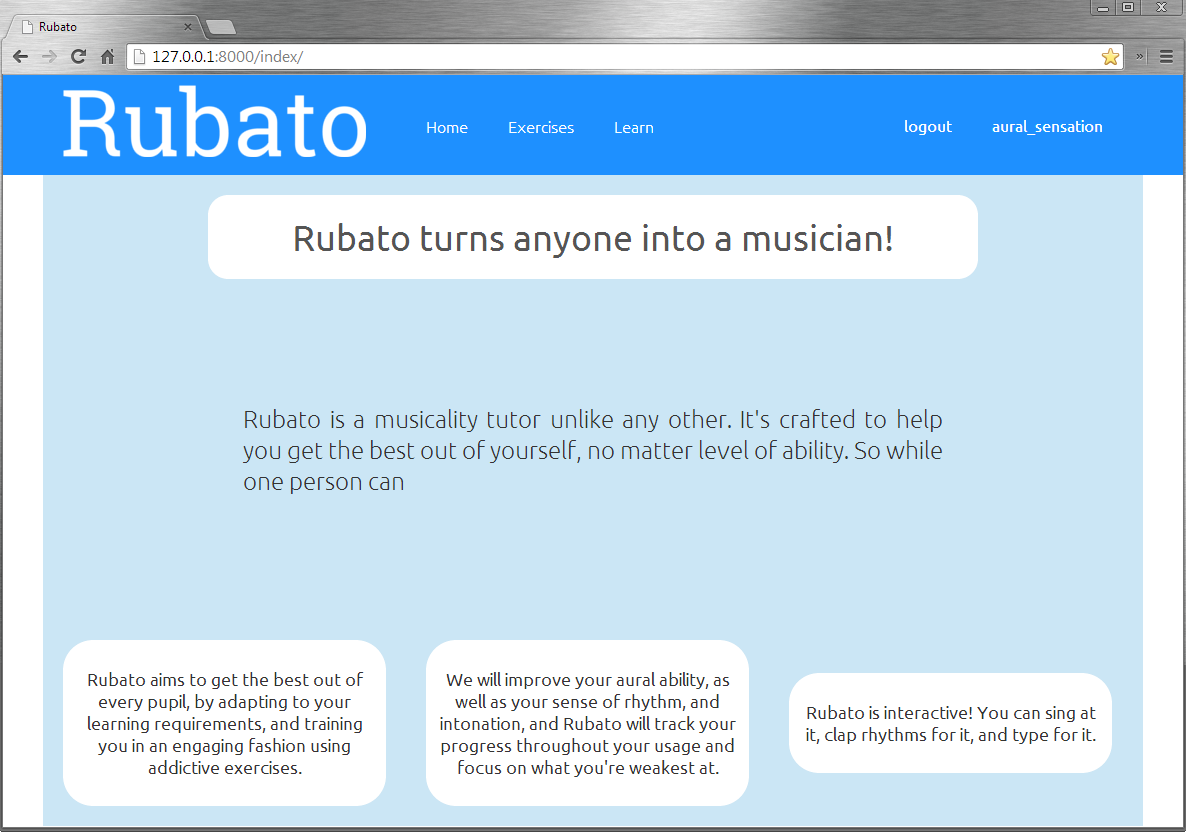
\includegraphics[scale=0.4]{webpage.png}
	\caption{The home page of the website}
\end{figure}

\subsection{Application flow}
	\subsubsection{Django web framework}
		\paragraph{Views}
		
		\paragraph{Models}
		Django interfaces with the database through Models. An example of this is the IntervalScore model below. This particular model stores all the information about a user's attempt at singing an interval in the interval training exercise.
		
		\begin[language = python]{lstlisting}
		class IntervalScore(models.Model):
   			interval = models.ForeignKey(Interval) 
    		timestamp = models.DateTimeField(auto_now_add=True)
    		score = models.FloatField();
		    user = models.PositiveIntegerField();
		    def __str__(self):
        		return " Score: " + str(self.score) + " for" + self.interval.name + " with user id: " + str(self.user)

		\end{lstlisting}
		The interval field represents the interval that the user has attempted, the timestamp tells us when it was attempted, and the score field tells us the calculated score for that attempt (it will be explained how this metric is derived in "Measuring user ability")
		
\section{Pitch Detection}
\par Pitch detection is an important part of the exercises, and as such, robust pitch detection has been an important feature in the development of this program. 
\par Most existing pitch detection algorithms are based on real-time applications, i.e. where audio captured from a microphone is analysed and the pitch is displayed as a constantly updating function of the audio signal. This is useful for applications like guitar tuning, where you need near instant feedback, and you can be sure that the pitch you are inputting is fairly constant. 
\par With analysis of pitch in the human voice however, the problem is that even with well trained singers, the pitch of a note can vary quite considerable over a 2 second period, due to vibrato\footnote{Vibrato is the musical technique of intentionally oscillating the pitch of the note around a fixed point.}, or other causes that can be hard to pick up just by listening to yourself, so it is not always trivial to determine one pitch to summarise a sample of a single held note, and indeed, often not appropriate to do so if the singer cannot even stay on the same note for that short period of time, and wobbles around the note inconsistently.
\par It is with this in mind that I have developed a Segmented Pitch Detection Algorithm, that can accurately determine the pitch of a 2-3 second sample of singing.

\subsection{Segmented Pitch Detection Algorithm}
The principle of the Segmented Pitch Detection Algorithm is relatively simple: A given audio sample is split into several segments, pitch detection is run on each segment, and then the segments are analysed to calculate pitch. I have also employed several error detection/correction methods that are detailed below.
\begin{figure}
	\centering
	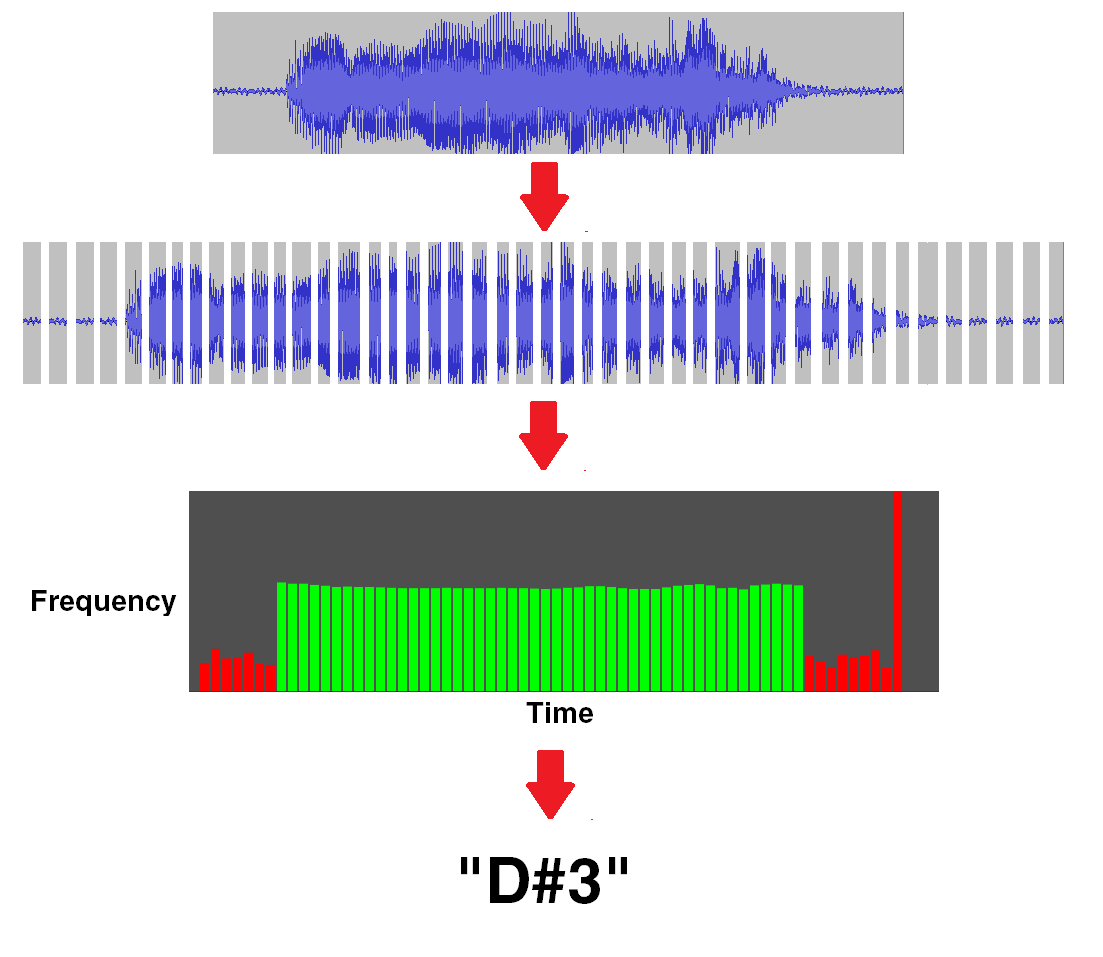
\includegraphics[scale=0.5]{segmented_autocorrelation.png}
	\caption{An illustration of how Segmented Autocorrelation works}
\end{figure}

\subsection{Breaking it apart}

\subsubsection{Choosing a segment size}
\par Most PC microphones sample audio at either 44,100Hz or 48,000Hz, as these ensure that the full 20KHz spectrum of human hearing can be recorded due to the Nyquist–Shannon sampling theorem (see Background section 2.5). For the sake of simplicity we will assume a sample rate of 48,000Hz for this report, though the program can handle either rate.
\par The human vocal range defined in section 2.4.2 was E2 - C6, which corresponds to a frequency range of ~80-1000hz\cite{scientificPitchTable}. To calculate the number of samples at either end of the range: 
 		 \[48000\div 96 = 600 \text{ samples}\] 
		 \[48000\div 1000 = 48 \text{ samples}\]
		
\par In order for our autocorrelation algorithm to work, it is  necessary to take a segment size at least twice that of the lowest frequency we wish to sample.
This is because in autocorrelation, we must compare the signal with an offset version of itself, and this score is maximal with an offset equal to the period of the signal. Therefore, in our example, if we use anything less than a 1200 sample size and are trying to detect a 96Hz signal, we won't even be able to autocorrelate on a full period. [DIAGRAM illustrating how you only compare half a period of you use a 900 sample segment] I have therefore decided to use 1200 as the segment size. Increasing this number results in a higher quality analysis per segment, but the trade-off is that segments per second decreases, meaning you are sacrificing granularity of change of pitch over time. [DIAGRAM of debug freqs graph at differing window sizes.

\subsubsection{Autocorrelation}
The algorithm for the pitch analysis for individual segments is the autocorrelation algorithm outlined in the first chapter. It is fast, simple to implement, and we don't mind so much about errors due to the fact that it's not a real-time implementation. This means we can look at each segment in the context of the whole recording, and run error correction algorithms outlined below if we do encounter any dodgy pitch readings.

\subsubsection{Enhancing the results: Quadratic Interpolation}
With autocorrelation, one inherent limitation is the granularity of the detected pitch.
Let's say a we are trying to identify a sung D4. This has a frequency of 293.66Hz and will therefore correspond to a lag of \(48,000Hz/293.66Hz = 163.45 \text{samples}\). Our algorithm at present does not have a way of dealing with fractions of a sample, so at best we will detect 163 or 164 samples. This lack of precision in this case will cause an error of roughly \(\pm 5 \text{cents}\), which isn't too bad. The problem however becomes more significant as we detect notes with higher frequencies, as these notes will correspond to smaller lag times, and thus a discrepancy in lag detected will correspond to a more noticeably error in pitch detection.

One way to solve this problem is quadratic interpolation. The idea is to take three points and built a guadratic curve between them. This is a good approximation of the waveform of an autocorrelation function



\subsection{Detecting errors}
There are 2 primary methods of detecting errors after autocorrelation has been performed.
Firstly, we		
\subsubsection{Median Filtering}
Median filtering is a noise reduction process used when sharp spikes occur in a signal. It works using a sliding window algorithm, applying a median filter to all the elements in a grid. The code below describes an implementation in Javascript, and Figure 3.2 gives a visualisation of how it works. 
For this application, the median filter is more appropriate than the more standard moving average filter, as it it non-linear meaning that large spikes will be completely removed, not just smoothed over.
I apply the median filter straight 
\begin{lstlisting}
function medianFilter(signal,window_size){
    var medians = new Array(signal.length);
    for (var i = mid; i<signal.length-mid; i++){
        var mid = Math.floor(window_size/2);
        var startIndex = i - mid;
        var median_window = new Array(windown_size);
        for (var j = 0; j <window_size; j++){
            median_window[j] = signal[startIndex + j];
            }
        }
        medians[i] = median(median_window);
    }
    return medians;
}
\end{lstlisting}

In my implementation I use window size 3, as large spikes of this sort are fairly rare, and when they do occur they're usually only 1 segment wide.

\begin{figure}
	\centering
    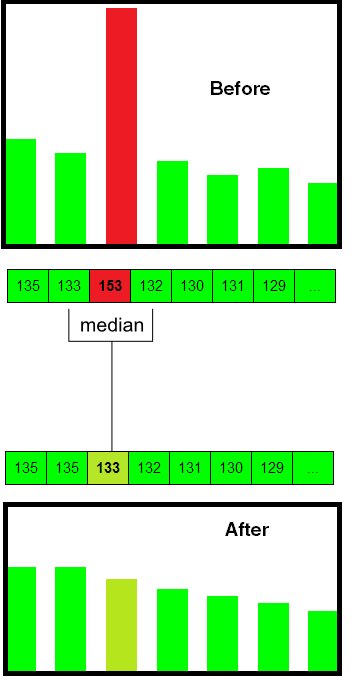
\includegraphics[scale=0.7]{median_demonstration_tall.png}
	\caption{A visualisation of the median filter with window size 3}
\end{figure}


\subsubsection{Amplitude filtering}
A typical audio sample will have junk data at either end of the recording as the user prepares to sing after activating the microphone, and then leaves the microphone running for a fraction of a second after singing. Amplitude filtering is designed to detect where the edges of the useful data are, and cut them off.

During the autocorrelation, as well as calculating the pitch for each segment, we also calculate it's amplitude using root mean square (RMS). It is preferable to use RMS to the conventional peak amplitude method normally used on audio signals, as our window size is sufficiently high that a spike in a given segment due to external noise could cause the amplitude value to be too high. RMS should avoid this as it takes an average over a given sample. The RMS amplitude is calculated using the following algorithm:
 \[\sqrt{\sum_{i=1}^{n} s_i^2/n}\], where \(n\) is the number of samples in the segment, and \(s_i\) is the i-th sample in the segment. After analysing all segments we end up with a result similar to that shown in Figure 3.3, with a block of loudness surrounded by two blocks of quietness.

\subparagraph{Microphone calibration}
To make sense of this, we have to work out what data should be accepted, and what should be rejected as too quiet to contain valid pitch data. This is done through calibration: The first time the user opens an exercise that uses microphone data, the program records a 2 second sample and segments it similarly to the preprocessing of the autocorrelation method. The minimum amplitude of all segments is then taken as the calibration value, \(a_0\).
When determining which segments to cut off in the amplitude filtering stage, we discard all segments with \(\text{amplitude} < 2 \times a_0\). This value has been determined empirically to be a reasonable threshold for minimum amplitude

\section{Putting it together}
\subsubsection{Rolling standard deviation}
In order to determine which blocks of data


\begin{figure}
	\centering
    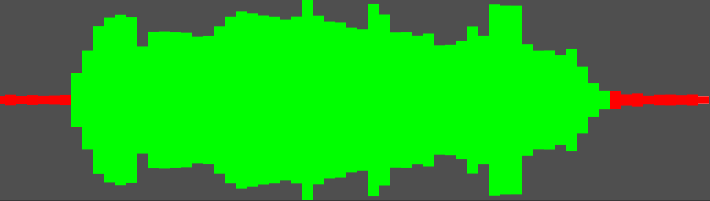
\includegraphics[scale=0.7]{amplitude_filtering.png}
	\caption{Amplitude filtering}
\end{figure}
\section{Measuring user ability}

User ability is measured through a level system. Every user has a level value assigned to each exercise they attempt, as well as for each category, and every user has an overall level also. Users with a high level will not have to start from the beginning when attempting new exercises. 

All users start at at level 1 when they sign up.

To increase their level, the user has to complete exercises correctly. As their level increases, the exercises adapt and get harder.

Measuring user ability is achieved by assigning a score to every \bsq{attempt} at a certain exercise. These scores are then processed by the server to determine:
	\begin{itemize}
		\item Whether the user should be levelled up.
		\item What questions it is best to ask them next.
	\end{itemize}

\subsection{Interval training}

The scoring system for interval training is as follows:

\[\text{difference} = |P_\text{actual}- P_\text{target}|\]
\[\text{perfect\_score} = 0.1 \]
\[\text{distance\_from\_perfect} = \text{max}(\text{difference}-\text{perfect\_score},0)\]
\[\text{score} = \text{max}(1 - \text{distance\_from\_perfect},0)\]

Intuitively, this means that any interval attempt less than 0.1 semitones from the actual pitch is classed as a perfect score, and anything over 1.1 semitones away is classed as a zero,with values between those 0.1 and 1.1 semitones determined by linear interpolation.

Every time the 


\subsection{Note from chord}
\subsection{Beat reproduction}

\section{Adapting to user ability}
Discussion of the adaptive element of the program for different exercises.
